%%% This LaTeX source document can be used as the basis for your technical
%%% report. Intentionally stripped and simplified
%%% and commands should be adjusted for your particular paper - title, 
%%% author, citations, equations, etc.
% % Citations/references are in report.bib 

\documentclass[conference]{acmsiggraph}

\usepackage{graphicx}
\graphicspath{{./images/}}
\newcommand{\figuremacroW}[4]{
	\begin{figure}[h] %[htbp]
		\centering
		\includegraphics[width=#4\columnwidth]{#1}
		\caption[#2]{\textbf{#2} - #3}
		\label{fig:#1}
	\end{figure}
}

\newcommand{\figuremacroF}[4]{
	\begin{figure*}[h] % [htbp]
		\centering
		\includegraphics[width=#4\textwidth]{#1}
		\caption[#2]{\textbf{#2} - #3}
		\label{fig:#1}
	\end{figure*}
}


\usepackage{lipsum}

\TOGonlineid{45678}
\TOGvolume{0}
\TOGnumber{0}
\TOGarticleDOI{1111111.2222222}
\TOGprojectURL{}
\TOGvideoURL{}
\TOGdataURL{}
\TOGcodeURL{}

\title{An OpenGl Desert Scene}

\author{Sam Serrels\\\ 40082367@napier.ac.uk \\
Edinburgh Napier University\\
Computer Graphics (SET08116)}
\pdfauthor{Sam Serrels}

\keywords{OpenGL, GLSL, Graphics, SSBO, Reflections}

\begin{document}

\teaser{
   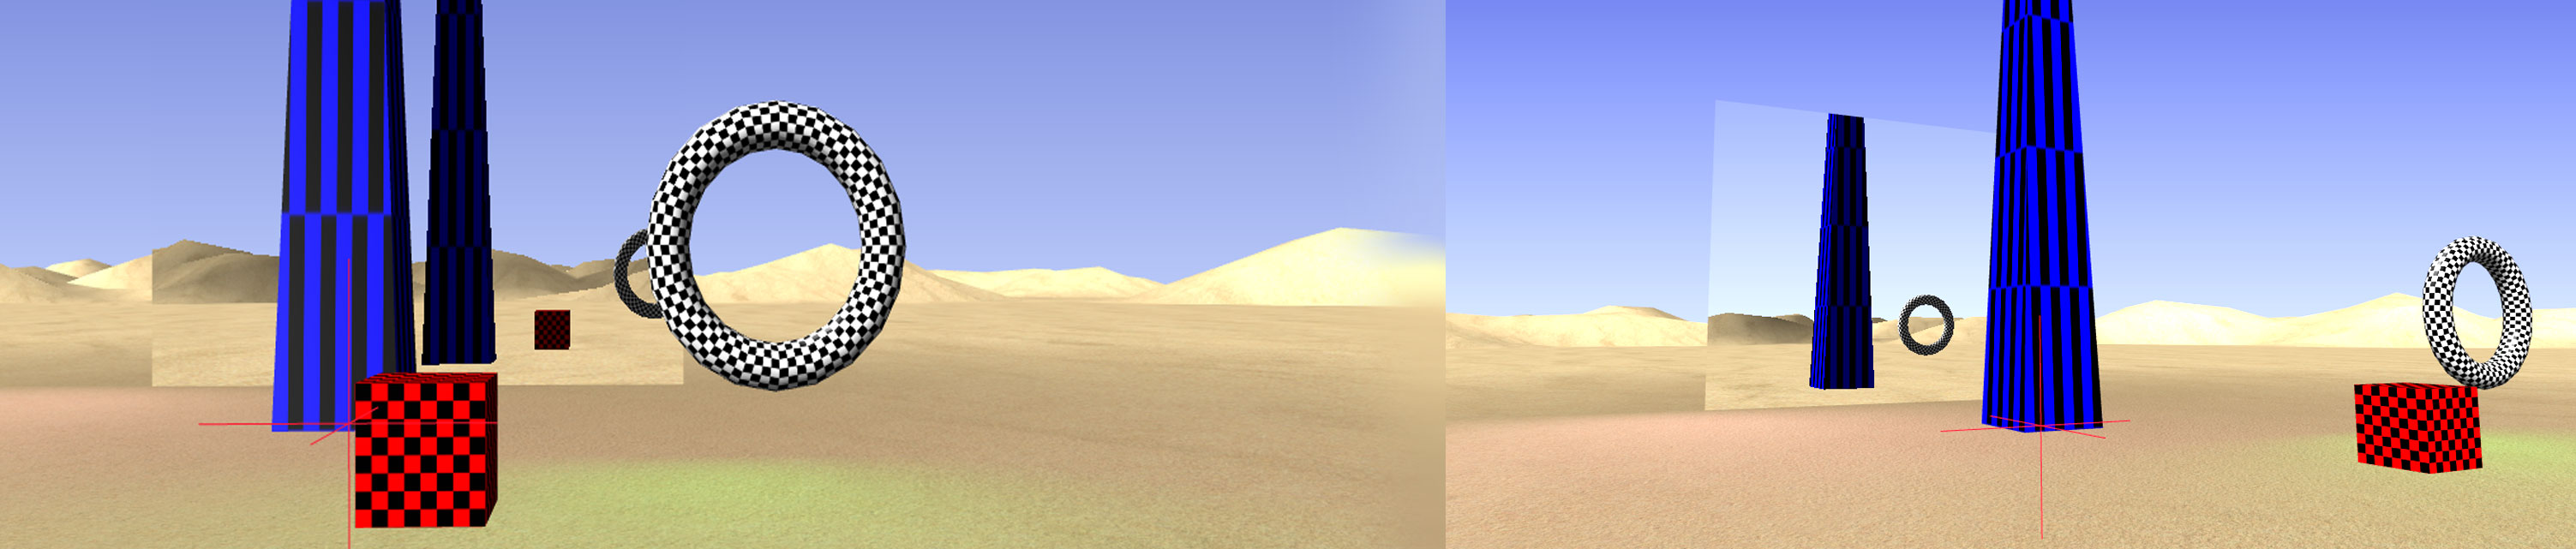
\includegraphics[height=1.5in]{images/sampleteaser}
   \caption{Project screenshot}   
 }		

\maketitle

\begin{abstract}
This project aims to develop a Real-time 3D graphics scene, with an emphasis on high aesthetic quality. The scene will use a pre-written OpenGL render framework to save development time for producing graphical effects. This project aims to also look into the cutting edge features available in the newest OpenGL standards and investigate the performance benefits of such features.
\end{abstract}

\keywordlist
%\copyrightspace

\section{Introduction}

\figuremacroW
{witness}
{Project Inspiration - The Witness}
{\protect\cite{Witness}}
{1.0}

\paragraph{Project Aims}
The setting for the project scene is a Desert. Although not a visually busy scene, a desert provides vibrant and harsh lighting, interesting landscape and plenty of opportunity to squeeze more visual fidelity out of a small amount of scene elements.
Using a multitude of texture effects, such as bump and parallax mapping, blend maps and level-of-detail, this project plans to bring life to even the most basic of objects, like sand on the ground.

\paragraph{Sky}
With the wide open vita of a desert plain, the sky takes center stage and is the most important visual cue to selling the realism of the scene. This project aims to have a fully dynamic and procedural sky system, without relying on static textures. This will allow for a time-of day system and full control of elements such as clouds and sun position.

\paragraph{Water}
The centrepiece of the scene will be a water feature of some kind, providing a contrast against the dry desert and visually interesting element in it's own right. Reflections, waves using distortion maps, refraction, and particle effects will be used to provide realistic looking water. 

\section{Background / Related Work}
\figuremacroW
{specops}
{Spec Ops: The Line}
{\protect\cite{spec}}
{1.0}
Desert scenes are not uncommon to video games, the  simplicity of the landscape was a large bonus to performance limited software.
Older games (pre DirectX 9), could get away with a simple ground mesh, a single sand texture and an interesting skybox, and this would be considered a sufficiently detailed scene for the time. See Figure: \ref{fig:GuildWars}
\\
As the graphical power of computer increased, the challenges to make a realistic desert increased dramatically, the standard of games required more than just a barren wasteland. Buildings, foliage, human characters and interesting landscape were needed and now the scene is just as complex as any other environment.
Some modern games have taken up the challenge to model sand behaviour, as a very simple fluid dynamics system to add life to a scene. Sandstorms are a popular feature as they offer the valuable benefit of obscuring level elements, these elements now do not have to be rendered, therefore increasing performance.

\figuremacroW
{GuildWars}
{Project Inspiration - Guild Wars}
{\protect\cite{GuildWars}}
{1.0}

\paragraph{Sky}
Procedural skys have been used in games for many years, the choice to use them depends on the needs of the game.  Games that have aim to have a more living environment are the primary uses for procedural skies, in other games if a static image is sufficient, then a simple texture is used.
 
\figuremacroW
{fallout3}
{Procedural Sky - Fallout 3}
{\protect\cite{fallout3}}
{1.0}

\section{Implementation}

\subsection{Sky}
Rendering the sky was achieved by rendering a single screen sized quad to the screen, set at a maximum depth to place it behind all the level elements. Calculations based on the players view matrix and the projection matrix, result in two values 

\figuremacroW
{reflections}
{Refection Camera position}
{\protect\cite{Riemer}}
{1.0}


\figuremacroW
{front-Buffer}
{Rendered Scene}
{Mirror Outline overlay for clarity}
{1.0}


\figuremacroW
{ref-Buffer}
{Refection Camera View}
{UV coordinates shown, this is the area that will be rendered on the mirror quad}
{1.0}

\section{Evaluation}

\paragraph{Scope}
The results of the project have been inconclusive in determining the performance benefits of physics optimisation across multiple platforms. The main shortcoming has been the Playstation 3 portion of the project. Due to unforeseen technical problems and the time constraints of the project, the support for the Playstion 3 could not be completed to a level which would result in usable results. Issues with the rendering framework and subtle differences in the maths libraries across the two platforms caused substantially more time spent on fixing code issues than developing features.

\paragraph{Playstation 3 results}
Unfortunately, optimising the code for the strengths of the Playstation 3, such as subdividing the work to the separate SPU processors was not achieved. Rendering issues caused the final output of the project to be generally unviewable on the Console.

\paragraph{PC results}
The results of the simulation were more positive on the PC architecture. The simulation runs well and without any major issues, major features detailed in the original design have been omitted due to time constraints. Visually the program is basic, without any graphics embellishments to bring the output closer to the original design vision.

\section{Future Work}
The primary focus for future work would be to fix and complete the Playstation code to bring it upto par with the PC code, then other features can be worked on. Firstly, dynamic control of simulation variables at runtime, allowing the user to interact with the simulation while it running. The User should be able to adjust parameters such as the  size of the world, the attributes of the spacial partitioning, and the ability to create and remove balls at will.\\
More complex collision shapes would be the next area of work, followed by rendering improvements.

\bibliographystyle{acmsiggraph}
\bibliography{report}


\end{document}